\chapter{Mathematical Foundations of Classification Model}



\section{Probability Distribution}

A probability distribution is the information of how likely a random variable or set of variables is to take each of its possible states. The way the probability distribution is described depended on whether the variables are discrete or continuous. A discrete random variable has finite or countably infinite number of states. \parencite[Page 54]{Goodfellow-et-al-2016}.  

In this project, the random variables are vector-valued product features denoted as $ \textbf{x} $ and its value as $ x $. The probability that variable $\textbf{x} = x$ is denoted by $ P(x) $, with a probability of 1 indicating that $\textbf{x}-x$ is certain and probability of 0 indicating an impossible event \parencite[Page 55]{Goodfellow-et-al-2016}.


The probability values ranging between 0  and 1 are called \acf{PMF} denoted as capital $ P $. To ensure that \acs*{PMF} provides valid probabilities the function $P$ must satisfy following properties.


\begin{itemize}
    \item Domain of PMF must be defined for all possible states of random variable $x$. It should specify probabilities for each value $x$. For example, of the variable of vector representation of product name ``X'' the $P$ must be defined for all categories.
    \item The $ P(x) $ must satisfy $0 \leq  P(x) \leq  1$.
    \item Impossible events have probability 0.
    \item Certain events have probability 1.
    \item Normalization property indicating sum of all probabilities equals to 1.
\end{itemize}


\begin{table}[H]
    \centering
    \begin{tabular}{ccccccc}
        \hline
        $x$ & $x_1$ & $x_2$ & $x_3$ & $\dots$ & $x_n$ \\
        \hline
        $P(x)$ & $P_1$ & $P_2$ & $P_3$ & $\dots$ & $P_n$ \\
        \hline
    \end{tabular}
    \caption{Probability Distribution $P(x)$ for Random Variable $x$}
    \label{tab:probability-distribution}
\end{table}


where \(P_i > 0\), \(i \equiv 1\) to \(n\) and \(P_1 + P_2 + P_3 + \ldots + P_n = 1\) \\

\subsection*{Multinoulli Distribution or Categorical Distribution}

Multinoulli or Categorical distribution is a type of probability distribution over a single discrete variable with $ k $ different states or categories, where $ k $ is finite and probability of each category is separately specified.

\begin{itemize}
    \item A multinoulli distribution is parametrized by a vector $\mathbf{p} \in [0, 1]^{k-1}$, where each element of $\mathbf{p}$ represents the probability of the $i$-th state. 
    \item  The probability of the final, $k$-th state is given by $1 - \sum_{i=1}^{k-1} p_i$. 
    \item  $\sum_{i=1}^{k-1} p_i \leq 1$ hence, the probabilities do not exceed 1. 
\end{itemize}



Multinoulli distributions are often employed to model distributions over categories of objects. In this context, we do not assume that state 1 has a numerical value of 1, and so forth. The values in $\mathbf{p}$ represent probabilities associated with different categories or states, and they do not carry a numerical interpretation.

Moreover, when working with multinoulli-distributed random variables, it is typically unnecessary to compute expectations or variances since these distributions are used to describe categorical outcomes where numerical operations may not be meaningful \parencite[Page 60,61]{Goodfellow-et-al-2016}. 


\section{Softmax}

The softmax function is often used to predict the probabilities associated with a multinoulli distribution \parencite[Page 79]{Goodfellow-et-al-2016}.

\begin{align}
    \text{Softmax}(x_i) = \frac{{\exp(x_i)}}{{\sum_{j=1}^n \exp(x_j)}} \label{eq:softmax_matth}
\end{align}

Equation \ref{eq:softmax_matth} is the formula for Softmax function. It applies the standard exponential function to each element $ x_i $ of the input vector $ \mathbf{x} $  and normalizes these values by dividing by the sum of all these exponential. 

\begin{lstlisting}[language=Python,caption={Python example for softmax},label=code:sample_softmax]
    >>> import numpy as np
    >>> a = [1.0, 2.0, 3.0, 4.0, 1.0, 2.0, 3.0]
    >>> np.exp(a) / np.sum(np.exp(a))
    array([0.02364054, 0.06426166, 0.1746813 , 0.474833  , 0.02364054,
           0.06426166, 0.1746813 ])
    >>> sm_val =np.exp(a) / np.sum(np.exp(a))
    >>> np.sum(sm_val)
    0.9999999999999999
    >>>
\end{lstlisting}

Listing \ref{code:sample_softmax} is an example of applying Softmax function to an array of positive integers. It is important to note that the sum of all the softmax value is approximately equal to 1.  The output has most of its weight where the ``4'' was in the original input. This is what the function is normally used for: to highlight the largest values and suppress values which are significantly below the maximum value.



\subsection*{Why to apply log to Softmax function } \label{sec:Logsoft}

 
\begin{align}
    \log(\text{Softmax}(x_i)) = \log\left(\frac{{\exp(x_i)}}{{\sum_{j=1}^n \exp(x_j)}}\right) \label{eq:log_softmax}
\end{align}

Equation \eqref{eq:log_softmax} shows the logarithm of the Softmax function applied to the element \(x_i\) in the vector \(\mathbf{x}\). 

Applying logarithm to the fraction: 
\begin{align}
    \log\left(\frac{a}{b}\right) = \log(a) - \log(b)
\end{align}

Substituting \(a = \exp(x_i)\) and \(b = \sum_{j=1}^n \exp(x_j)\) in equation \eqref{eq:log_softmax}, we get:

\begin{align}
    \log(\text{Softmax}(x_i)) = \log(\exp(x_i)) - \log\left(\sum_{j=1}^n \exp(x_j)\right)
\end{align}

\begin{itemize}
    \item Reduce large numbers:  The softmax function normalizes any value from [-infy, +infy] by applying an exponential function. Exponential functions can lead to a very large numbers, resulting in  Nan as output. Applying logarithm effectively reduce these large numbers to manageable range.
    \item Numerical Stability: When dealing with very small probabilities, the product of multiple probabilities can become exceedingly close to zero, leading to numerical underflow. Similarly, when dealing with very large probabilities, the product can exceed the representation range of standard floating-point numbers, causing numerical overflow. By taking the logarithm, these issues are avoided, and the values are represented in a more stable and manageable range \parencite[Page 79]{Goodfellow-et-al-2016}.
    
    \item Log Probabilities and Addition: Log probabilities are additive when events are independent.\\ For example, if we have two independent events \(A\) and \(B\) with probabilities \(P(A) = p\) and \(P(B) = q\), the probability of both events occurring (\(P(A \cap B)\)) is \(P(A) \times P(B) = p \times q\). Taking the logarithm, we get \(\log(P(A \cap B)) = \log(p \times q) = \log(p) + \log(q)\). This additive property simplifies calculations involving multiple independent events.

    \item Logarithms and Multiplication: Logarithms convert multiplication to addition. Probabilities of independent events,  represented as \(P(A \cap B \cap C \cap \ldots)\). Logarithm of the product of these probabilities simplifies the computation to a sum. 
\end{itemize}

\section{ \acs*{RNN} - Forward and Backward Propagation}

\acfp{RNN} \parencite{Rumelhart.1986} is best suited for machine learning problems that involve sequential data and use patterns to predict the output. A recurrent neural network is specialized for processing sequence of values $ x^{(1)},\ldots,x^{(t)}$.

\begin{figure}[H]
    \centering    
    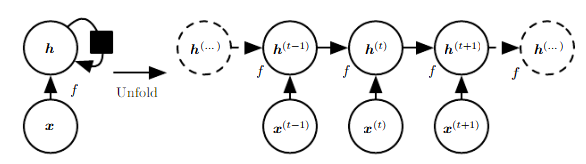
\includegraphics[scale=0.9]{rnn_wno.png}
    \caption{A \acl*{RNN} with no output \parencite[Page 370]{Goodfellow-et-al-2016}}
    \label{fig:RNN without output}
\end{figure}


\begin{align}
    h^{(t)} = f(h^{(t-1)}, x^{(t)}; \theta)
 \end{align}

Properties of a RNN are as follows \parencite[Chapter 10]{Goodfellow-et-al-2016}:- 
\begin{itemize}
    \item Graph un-rolling and parameter sharing.
    

    


\end{itemize}

This machine learning algorithm store information of previous states and holds the memory. 




\section{Summary}

In this chapter, the mathematical theories and formulas related to multi level classification task is described. Author discusses the approach for numerical stability to avoid overflow and underflow of value resulting into a not-a-number values. In this chapter, an overview of the Probability Distribution and one of its type Multinoulli Distribution is given. Author illustrates the relationship between the task of product feature classification into category and the mathematical formulas.  